
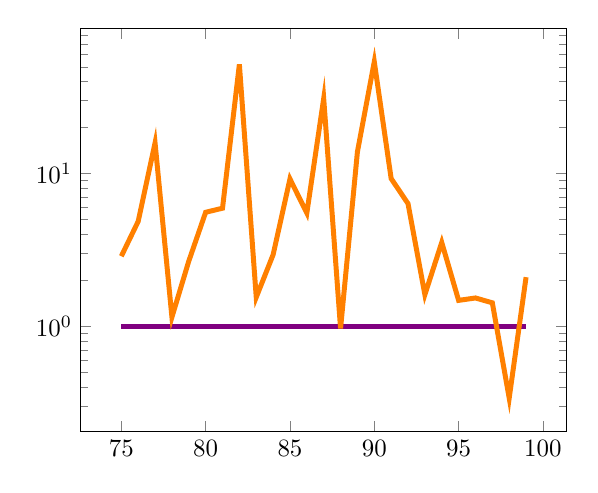
\begin{tikzpicture}[scale=0.9]
\begin{semilogyaxis}
\addplot[color=violet,line width=2pt] coordinates {(75,1.0)(76,1.0)(77,1.0)(78,1.0)(79,1.0)(80,1.0)(81,1.0)(82,1.0)(83,1.0)(84,1.0)(85,1.0)(86,1.0)(87,1.0)(88,1.0)(89,1.0)(90,1.0)(91,1.0)(92,1.0)(93,1.0)(94,1.0)(95,1.0)(96,1.0)(97,1.0)(98,1.0)(99,1.0)};
\addplot[color=orange,line width=2pt] coordinates {(75,2.873175759272601)(76,4.859620272990034)(77,15.858963003267606)(78,1.146602789998144)(79,2.667575909639226)(80,5.572347647236092)(81,5.925875189215517)(82,51.831025951386586)(83,1.5477949890285654)(84,2.93690643493153)(85,9.206938066245588)(86,5.508301965820871)(87,30.969548530712164)(88,0.9665117816864832)(89,13.869858043497933)(90,53.903475409013915)(91,9.267499346783847)(92,6.3490669460059035)(93,1.6091565053616068)(94,3.535610762753156)(95,1.4762394440739843)(96,1.5308539466673166)(97,1.4227428530231392)(98,0.3385567932353906)(99,2.0942259754653945)};

\end{semilogyaxis}
\end{tikzpicture}
